% This is the results section og the report on homework-2.
% Author(s) : Vivek Kumar / Victor Charpentier
% Last Updated : 04/03/2018
%%%%%%%%%%%%%%%%%%%%%%%%%%%
\section{Results and Discussion}
The first result we present is that of cross-validation performed on the split data to determine the best for each prediction. The total train data (obtained from {\ttfamily train.csv}) was divided randomly into a 50:50 split. The cross-validation score chosen for comparison was mean-squared-error (MSE). The results for each are displayed in Table [\ref{tab:mse_cross_continuous}].
\begin{table}[H]
\centering
	\begin{tabular}{|c|c|c|c|}
	\hline
	Method & GPA MSE & Grit MSE & Material Hardship MSE\\
	\hline
	Random Forest Regressor	&	0.221031	&	0.153470	&	0.015116	\\
	AdaBoost Regressor		&	0.250311	&	0.156094	&	0.017874	\\
	LassoLarsCV				&	0.232776	&	0.153386	&	0.016869	\\
	ElasticNet				&	0.379290	&	0.252420	&	0.017385	\\
	Extra Trees Regressor		&	0.219626	&	0.162074	&	0.016035	\\
	MLP Regressor			&	157140	&	190226	&	305336	\\
	\hline
	\end{tabular}
	\caption{Mean-Squared-Error score for various methods obtained in cross-validation for continuous variables}
	\label{tab:mse_cross_continuous}
\end{table}
\vspace{-10pt}
\begin{table}[H]
\centering
	\begin{tabular}{|c|c|c|c|}
	\hline
	Method & Eviction MSE & Layoff MSE & Job Training MSE\\
	\hline
	Quadratic Discriminant Analysis	&	0.053004	&	0.119698	&	0.163054	\\
	Random Forest Classifier		&	0.042568	&	0.101568	&	0.122916	\\
	Adaboost Classifier				&	0.200811	&	0.224494	&	0.230679	\\
	MLP Classifier				&	0.051826	&	0.232274	&	0.232747	\\
	ExtraTreesRegressor		&	0.041886	&	0.102059	&	0.123275	\\
	\hline
	\end{tabular}
	\caption{Mean-Squared-Error score for various methods obtained in cross-validation for discrete variables}
	\label{tab:mse_cross_discrete}
\end{table}
Using the best method the leaderboard scores were :
\begin{align*}
\mathrm{GPA \ Score \ :} \ 0.36792  && \mathrm{Grit \ Score \ :} \ 0.21894  && \mathrm{Material \ Hardship \ Score \ :} \ 0.02531
\end{align*}
The bootstrapping was performed on the training data set to determine the minimum and maximum error obtained for each prediction. Here we have used RandomForestRegressor as the method for predicting the results. The results are plotted in the Figure [\ref{fig:bootstrapping}]. These results clearly show that there are multiple cases when the method is expected to fail. These cases, could be identified and further studied. The cases could be used to further train a more deep training data, say a neural network.\\
\begin{figure}[H]
\centering
\includegraphics[width=0.8\textwidth]{bootstrapping}
\caption{Bootstrapping results}
\label{fig:bootstrapping}
\end{figure}
Further to understand, which features were most important the {\ttfamily mutual\_info\_regression} from {\ttfamily feature\_seclection} of sklearn was used. The plot shows the mutual information between each feature and the target prediction shown in Figure [\ref{fig:mutual_info}]
\begin{figure}[H]
\centering
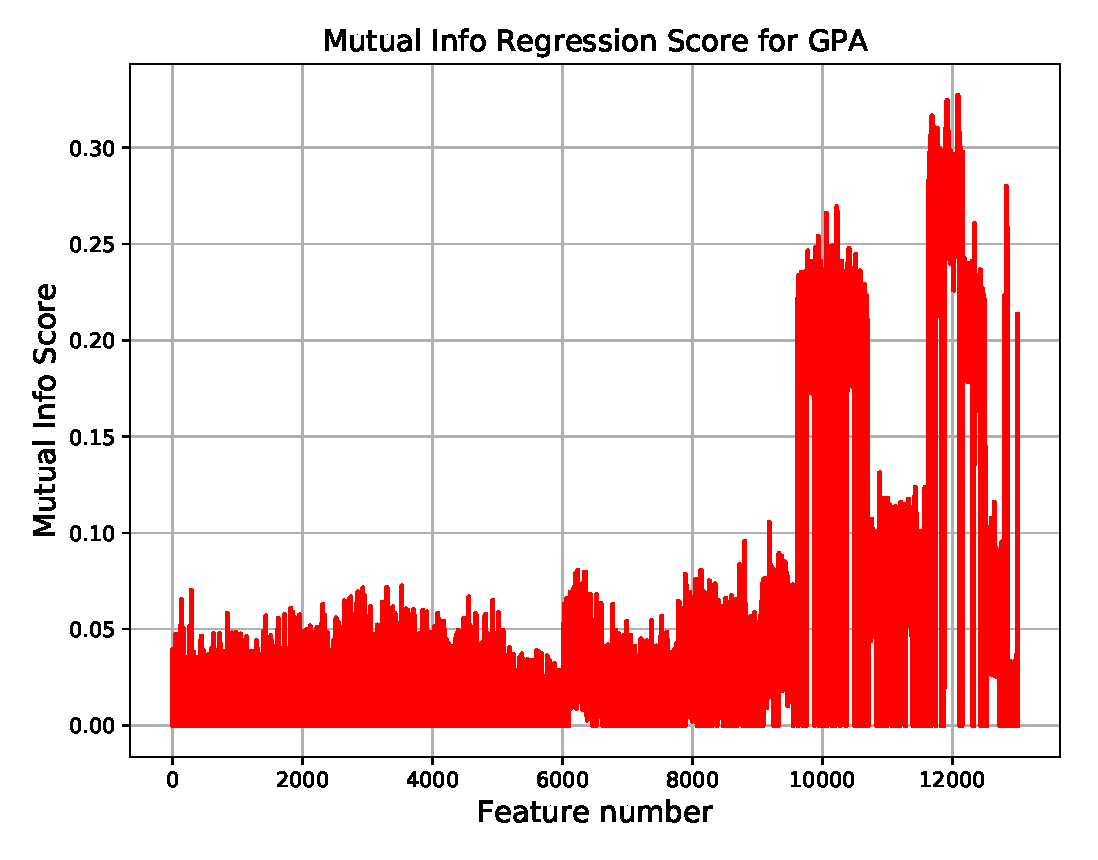
\includegraphics[width=0.49\textwidth]{feature_selection_gpa_scores}
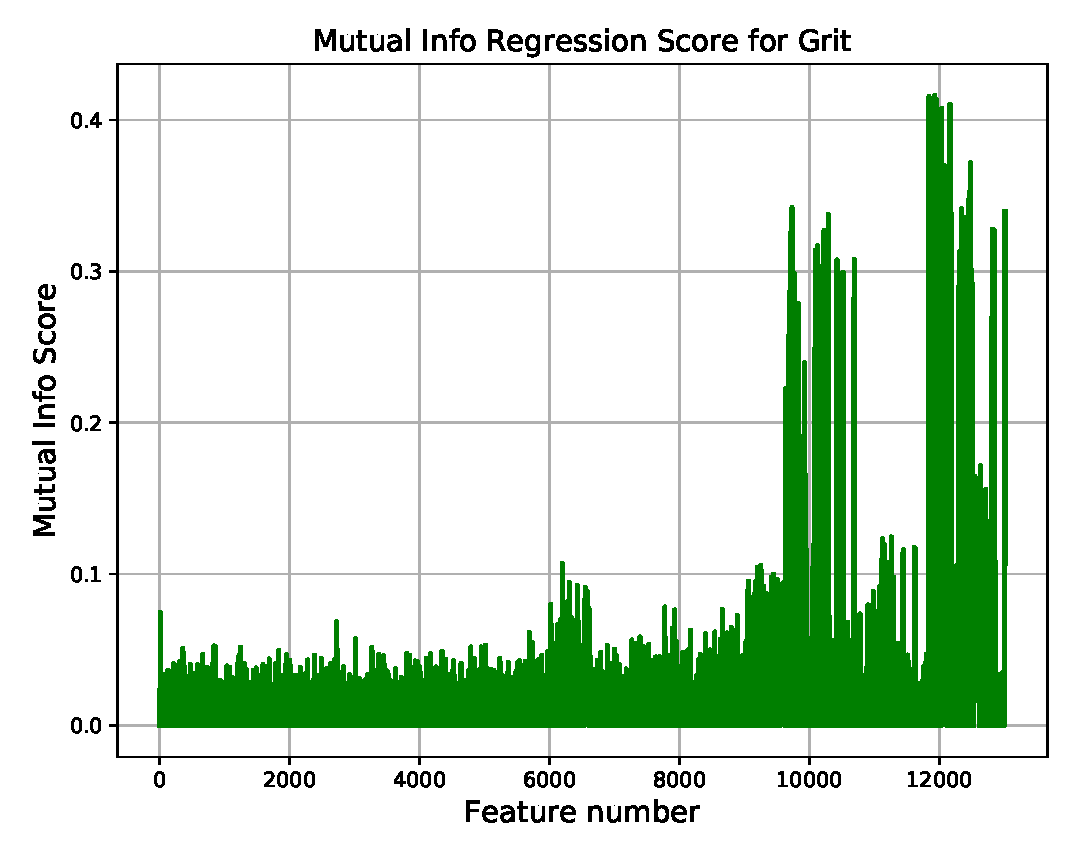
\includegraphics[width=0.49\textwidth]{feature_selection_grit_scores}
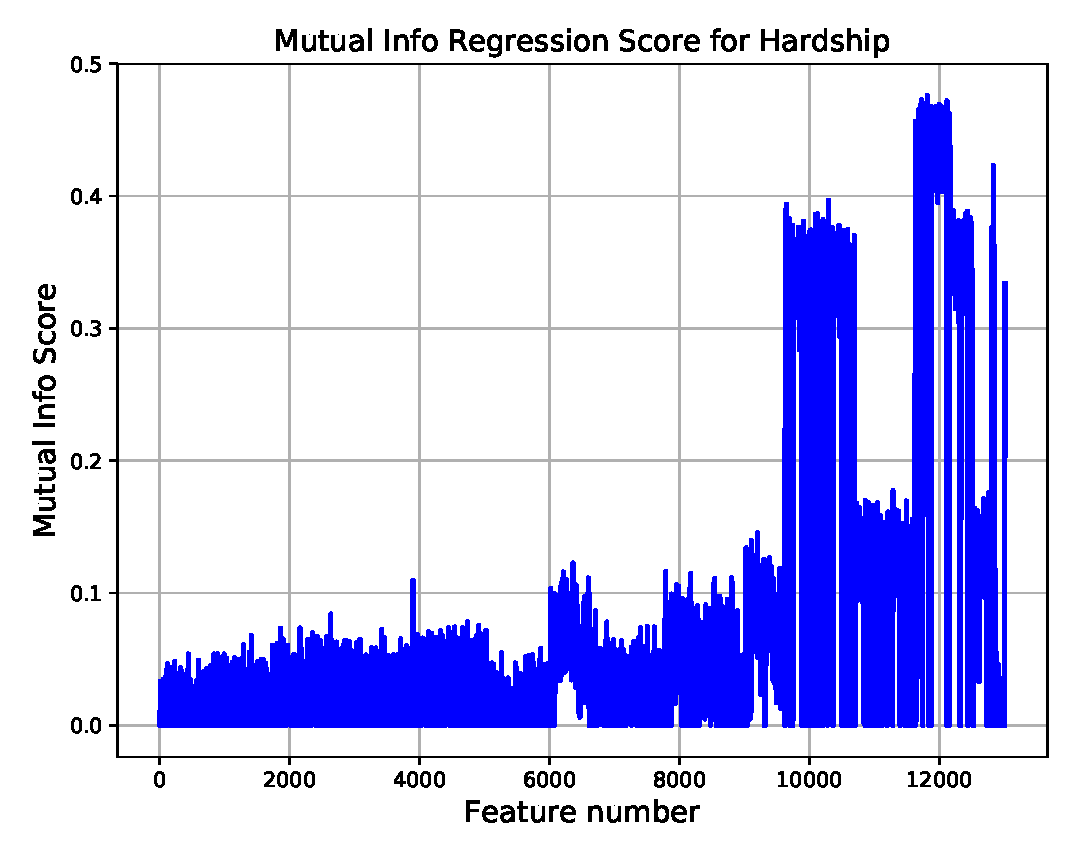
\includegraphics[width=0.49\textwidth]{feature_selection_hardship_scores}
\caption{Mutual Information Score for various parameters to predict}
\label{fig:mutual_info}
\end{figure}
We also employed the principal component analysis (PCA) for dimension-reduction. Instead of showing the individual results we compare how the methods performed when various feature selection or dimension reduction techniques were employed. Based on the figure [\ref{fig:mutual_info}] the mutual info score cutoff was set at 0.1. For PCA the features were selected so as to explain 99\% of the variance.
\begin{table}[H]
\centering
	\begin{tabular}{|c|c|c|c|}
	\hline
	Method & None & Mutual Info ($>$ 0.1) & PCA(99\% variance)\\
	\hline
	RandomForestRegressor	&	0.221031	&	0.226496	&	0.239838	\\
	AdaBoostRegressor		&	0.250311	&	0.240569	&	0.279977	\\
	LassoLarsCV				&	0.232776	&	0.233773	&	0.241419	\\
	ElasticNet				&	0.379290	&	0.245301	&	0.241284	\\
	ExtraTreesRegressor		&	0.219626	&	0.223951	&	0.239640	\\
	MLPRegressor			&	157140	&	51837	&	4.548522	\\
	\hline
	\end{tabular}
	\caption{Mean-Squared-Error score for GPA with and without dimension reduction/ feature-selection}
\end{table}
